% Options for packages loaded elsewhere
\PassOptionsToPackage{unicode}{hyperref}
\PassOptionsToPackage{hyphens}{url}
\PassOptionsToPackage{dvipsnames,svgnames,x11names}{xcolor}
%
\documentclass[
  12pt,
]{article}

\usepackage{amsmath,amssymb}
\usepackage{setspace}
\usepackage{iftex}
\ifPDFTeX
  \usepackage[T1]{fontenc}
  \usepackage[utf8]{inputenc}
  \usepackage{textcomp} % provide euro and other symbols
\else % if luatex or xetex
  \usepackage{unicode-math}
  \defaultfontfeatures{Scale=MatchLowercase}
  \defaultfontfeatures[\rmfamily]{Ligatures=TeX,Scale=1}
\fi
\usepackage{lmodern}
\ifPDFTeX\else  
    % xetex/luatex font selection
  \setmainfont[]{Times New Roman}
\fi
% Use upquote if available, for straight quotes in verbatim environments
\IfFileExists{upquote.sty}{\usepackage{upquote}}{}
\IfFileExists{microtype.sty}{% use microtype if available
  \usepackage[]{microtype}
  \UseMicrotypeSet[protrusion]{basicmath} % disable protrusion for tt fonts
}{}
\makeatletter
\@ifundefined{KOMAClassName}{% if non-KOMA class
  \IfFileExists{parskip.sty}{%
    \usepackage{parskip}
  }{% else
    \setlength{\parindent}{0pt}
    \setlength{\parskip}{6pt plus 2pt minus 1pt}}
}{% if KOMA class
  \KOMAoptions{parskip=half}}
\makeatother
\usepackage{xcolor}
\usepackage[lmargin=1in,rmargin=1in,tmargin=1in,bmargin=1in]{geometry}
\setlength{\emergencystretch}{3em} % prevent overfull lines
\setcounter{secnumdepth}{-\maxdimen} % remove section numbering
% Make \paragraph and \subparagraph free-standing
\ifx\paragraph\undefined\else
  \let\oldparagraph\paragraph
  \renewcommand{\paragraph}[1]{\oldparagraph{#1}\mbox{}}
\fi
\ifx\subparagraph\undefined\else
  \let\oldsubparagraph\subparagraph
  \renewcommand{\subparagraph}[1]{\oldsubparagraph{#1}\mbox{}}
\fi


\providecommand{\tightlist}{%
  \setlength{\itemsep}{0pt}\setlength{\parskip}{0pt}}\usepackage{longtable,booktabs,array}
\usepackage{calc} % for calculating minipage widths
% Correct order of tables after \paragraph or \subparagraph
\usepackage{etoolbox}
\makeatletter
\patchcmd\longtable{\par}{\if@noskipsec\mbox{}\fi\par}{}{}
\makeatother
% Allow footnotes in longtable head/foot
\IfFileExists{footnotehyper.sty}{\usepackage{footnotehyper}}{\usepackage{footnote}}
\makesavenoteenv{longtable}
\usepackage{graphicx}
\makeatletter
\def\maxwidth{\ifdim\Gin@nat@width>\linewidth\linewidth\else\Gin@nat@width\fi}
\def\maxheight{\ifdim\Gin@nat@height>\textheight\textheight\else\Gin@nat@height\fi}
\makeatother
% Scale images if necessary, so that they will not overflow the page
% margins by default, and it is still possible to overwrite the defaults
% using explicit options in \includegraphics[width, height, ...]{}
\setkeys{Gin}{width=\maxwidth,height=\maxheight,keepaspectratio}
% Set default figure placement to htbp
\makeatletter
\def\fps@figure{htbp}
\makeatother

% definitions for citeproc citations
\NewDocumentCommand\citeproctext{}{}
\NewDocumentCommand\citeproc{mm}{%
  \begingroup\def\citeproctext{#2}\cite{#1}\endgroup}
\makeatletter
 % allow citations to break across lines
 \let\@cite@ofmt\@firstofone
 % avoid brackets around text for \cite:
 \def\@biblabel#1{}
 \def\@cite#1#2{{#1\if@tempswa , #2\fi}}
\makeatother
\newlength{\cslhangindent}
\setlength{\cslhangindent}{0.5in}
\newlength{\csllabelwidth}
\setlength{\csllabelwidth}{3em}
\newenvironment{CSLReferences}[2] % #1 hanging-indent, #2 entry-spacing
 {\begin{list}{}{%
  \setlength{\itemindent}{0pt}
  \setlength{\leftmargin}{0pt}
  \setlength{\parsep}{1em}
  % turn on hanging indent if param 1 is 1
  \ifodd #1
   \setlength{\leftmargin}{\cslhangindent}
   \setlength{\itemindent}{-1\cslhangindent}
  \fi
  % set entry spacing
  \setlength{\itemsep}{#2\baselineskip}}}
 {\end{list}}
\usepackage{calc}
\newcommand{\CSLBlock}[1]{\hfill\break\parbox[t]{\linewidth}{\strut\ignorespaces#1\strut}}
\newcommand{\CSLLeftMargin}[1]{\parbox[t]{\csllabelwidth}{\strut#1\strut}}
\newcommand{\CSLRightInline}[1]{\parbox[t]{\linewidth - \csllabelwidth}{\strut#1\strut}}
\newcommand{\CSLIndent}[1]{\hspace{\cslhangindent}#1}

% TODO: Add custom LaTeX header directives here

\raggedright
\usepackage{ragged2e}  
\usepackage[hang,flushmargin,ragged]{footmisc}
\usepackage{sectsty}
\usepackage{titlesec}
\usepackage{tikz}
\usepackage{datetime}
\titlespacing*{\section}{0pt}{2\baselineskip}{\baselineskip}
\titlespacing*{\subsection}{0pt}{1\baselineskip}{0\baselineskip}
\titlespacing*{\subsubsectionfont}{0pt}{1\baselineskip}{0\baselineskip}        
\sectionfont{\normalfont\bfseries\normalsize\MakeUppercase}
\subsectionfont{\normalfont\bfseries\normalsize}
\subsubsectionfont{\normalfont\normalsize\itshape}   
\usepackage{caption}
\captionsetup[figure]{font=normal,labelfont=bf}
\captionsetup[table]{font=normal,labelfont=bf} 
 
\setlength{\parskip}{1.5em}

\usepackage{multicol}
\usepackage{etoolbox}
\usepackage{fancyhdr}
\usepackage{geometry}
\usepackage{fancyhdr}
 
\usepackage{booktabs}
\usepackage{chngcntr}
\usepackage{apptools}

\usepackage{lipsum}
\makeatletter
\@ifpackageloaded{caption}{}{\usepackage{caption}}
\AtBeginDocument{%
\ifdefined\contentsname
  \renewcommand*\contentsname{Table of contents}
\else
  \newcommand\contentsname{Table of contents}
\fi
\ifdefined\listfigurename
  \renewcommand*\listfigurename{List of Figures}
\else
  \newcommand\listfigurename{List of Figures}
\fi
\ifdefined\listtablename
  \renewcommand*\listtablename{List of Tables}
\else
  \newcommand\listtablename{List of Tables}
\fi
\ifdefined\figurename
  \renewcommand*\figurename{Figure}
\else
  \newcommand\figurename{Figure}
\fi
\ifdefined\tablename
  \renewcommand*\tablename{Table}
\else
  \newcommand\tablename{Table}
\fi
}
\@ifpackageloaded{float}{}{\usepackage{float}}
\floatstyle{ruled}
\@ifundefined{c@chapter}{\newfloat{codelisting}{h}{lop}}{\newfloat{codelisting}{h}{lop}[chapter]}
\floatname{codelisting}{Listing}
\newcommand*\listoflistings{\listof{codelisting}{List of Listings}}
\captionsetup{labelsep=period}
\makeatother
\makeatletter
\makeatother
\makeatletter
\@ifpackageloaded{caption}{}{\usepackage{caption}}
\@ifpackageloaded{subcaption}{}{\usepackage{subcaption}}
\makeatother
\ifLuaTeX
  \usepackage{selnolig}  % disable illegal ligatures
\fi
\usepackage{bookmark}

\IfFileExists{xurl.sty}{\usepackage{xurl}}{} % add URL line breaks if available
\urlstyle{same} % disable monospaced font for URLs
\hypersetup{
  pdftitle={Levy Economics Institute Working Paper Template},
  pdfkeywords={template, demonstration, Levywp, Quarto},
  colorlinks=true,
  linkcolor={blue},
  filecolor={Maroon},
  citecolor={Blue},
  urlcolor={Blue},
  pdfcreator={LaTeX via pandoc}}

% This is where the selected code should go

% Check if a title is provided
    \title{
        Levy Economics Institute Working Paper Template
        % Check if thanks is provided
            }

% Check if a subtitle is provided

% Set the authors

\author{
\textbf{Fernando Rios-Avila}
\footnote{The author thanks the Levy Economics Institute for financial
support.}\\
Levy Economics Institute\\[0.5cm]
\and 
\textbf{Author 2}
\footnote{The author thanks SOI for moral support.}\\
Some other Institute\\[0.5cm]
}

% Set the date
\date{June 4, 2024}


 
\begin{document}

\let\origfootnoterule\footnoterule
\renewcommand{\footnoterule}{}
\definecolor{levyblue}{RGB}{0, 70, 139}

\newgeometry{left=1in, right=1in, top=0.5in, bottom=0.5in} % change the margins


\begin{titlepage}

\begin{minipage}[t][0.70\textheight][t]{\textwidth} 
\renewcommand{\thempfootnote}{\fnsymbol{mpfootnote}} 
    \centering
    
\includegraphics[width=0.25\textwidth]{logo.png}\\[0.25cm]
    \textbf{\large{\textcolor{levyblue}{\fontspec{Arial}Working Paper No. ???}}}\\[0.3cm]

    \textcolor{lightgray}{\rule{0.8\textwidth}{0.5mm}}\\[0.5cm]

    \center{\textbf{Levy Economics Institute Working Paper
Template}} \\[0.5cm]
     
    \center{\textbf{by}} \\[0.5cm]
 % fill the vertical space

 
 \textbf{Fernando Rios-Avila}
 \footnote{The author thanks the Levy Economics Institute for financial
 support.}\\
 Levy Economics Institute\\[0.5cm]

 \textbf{Author 2}
 \footnote{The author thanks SOI for moral support.}\\
 Some other Institute\\[0.5cm]


 \center{June 4, 2024}

 \vfill 
 ~
 \end{minipage}
 

\center{\textcolor{lightgray}{\rule{0.8\textwidth}{0.5mm}}}\\[0.5cm]
        \vfill
    \begin{minipage}[b][0.20\textheight][b]{\textwidth}
    
        
        \begin{minipage}{\textwidth}
            \small
            The Levy Economics Institute Working Paper Collection presents research in progress by Levy Institute scholars and conference participants. The purpose of the series is to disseminate ideas to and elicit comments from academics and professionals.
        \end{minipage}\\[0.5cm]

        % Content of the bottom minipage (25% of the page)
        \begin{center}
        \fcolorbox{black}{lightgray}{
            \begin{minipage}{0.85\textwidth}
            \footnotesize
            Levy Economics Institute of Bard College, founded in 1986, is a nonprofit, nonpartisan, independently funded research organization devoted to public service. Through scholarship and economic research, it generates viable, effective public policy responses to important economic problems that profoundly affect the quality of life in the United States and abroad.
            \end{minipage}
        }
        \end{center} 
        \centering
        \vspace{0.5cm}
        \footnotesize   
        Levy Economics Institute\\
        P.O. Box 5000\\
        Annandale-on-Hudson, NY 12504-5000\\
        http://www.levyinstitute.org\\
        Copyright \textcopyright\ Levy Economics Institute 2024 All rights reserved\\
        ISSN 1547-366X

    \end{minipage}

    
\thispagestyle{empty}
\clearpage\pagenumbering{arabic}

\end{titlepage}

\let\footnoterule\origfootnoterule

\restoregeometry

\newpage



\textbf{ABSTRACT}

\vspace{1.5em}

\onehalfspace
This document is a template demonstrating the Levywp format. \lipsum[1]

\vspace{1.5em}

\textbf{KEY WORDS:} template, demonstration, Levywp, Quarto 

\textbf{JEL CLASSIFICATION:} A00, B00, C00

\newpage
\setstretch{1.5}
\section{Introduction}\label{sec-intro}

\emph{TODO} Create a template that demonstrates the appearance,
formatting, layout, and functionality of your format. Learn more about
journal formats at \url{https://quarto.org/docs/journals/}.

Zacharias et al. (2024), Masterson (2010), Rios‐Avila (2015)

\lipsum[1-2]

More text \footnote{This is a footnote.}

\lipsum[1] Here\footnote{This is a longer note with Text.\lipsum[1]}

\section{Level 1}\label{level-1}

\subsection{Level 1.0}\label{level-1.0}

\lipsum[1-2]

\subsection{Level 2}\label{level-2}

\lipsum[1-2]

\subsubsection{Level 3}\label{level-3}

\begin{table}[H]

\caption{\label{tbl-one}\textbf{Title here}}

\centering{

\centering
\begin{tabular}{|l|l|l|}
\hline
Header 1 & Header 2 & Header 3 \\ \hline
Cell 1   & Cell 2   & Cell 3   \\ \hline
Cell 4   & Cell 5   & Cell 6   \\ \hline
\end{tabular}

}

\end{table}%

\lipsum[1-2]

\begin{figure}

\caption{\label{fig-one}\textbf{Title here}}

\centering{

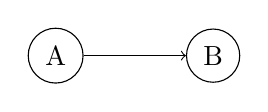
\begin{tikzpicture}
  \node[draw, circle] (A) at (0,0) {A};
  \node[draw, circle] (B) at (2,0) {B};
  \draw[->] (A) -- (B);
\end{tikzpicture}

}

\end{figure}%

This is indeed a lot of text that im now generating After you make your
repository a template, anyone with access to the repository can generate
a new repository with the same directory structure and files as your
default branch. They can also choose to include all the other branches
in your repository. Branches created from a template have unrelated
histories, so you cannot create pull requests or merge between the
branches. For more information, see ``Creating a repository from a
template.''After you make your repository a template, anyone with access
to the repository can generate a new repository with the same directory
structure and files as your default branch. They can also choose to
include all the other branches in your repository. Branches created from
a template have unrelated histories, so you cannot create pull requests
or merge between the branches. For more information, see ``Creating a
repository from a template.''

\section{References}\label{references}

\singlespacing

\phantomsection\label{refs}
\begin{CSLReferences}{1}{0}
\bibitem[\citeproctext]{ref-masterson2010}
Masterson, Thomas. 2010. {``Quality of {Match} for {Statistical}
{Matches} {Used} in the 1992 and 2007 {Limew} {Estimates} for the
{United} {States}.''} \{SSRN\} \{Scholarly\} \{Paper\}. Rochester, NY.
\url{https://doi.org/10.2139/ssrn.1680409}.

\bibitem[\citeproctext]{ref-rios2015}
Rios‐Avila, Fernando. 2015. {``Quality of {Match} for {Statistical}
{Matches} {Using} the {Consumer} {Expenditure} {Survey} 2011 and
{Annual} {Social} {Economic} {Supplement} 2011.''} Levy Economics
Institute Working Paper. Rochester, NY: Levy Economics Institute of Bard
College. \url{https://doi.org/10.2139/ssrn.2554089}.

\bibitem[\citeproctext]{ref-blsreport}
Zacharias, Ajit, Fernando Rios-Avila, Nancy Folbre, and Thomas
Masterson. 2024. {``Integrating {Nonmarket} {Consumption} into the
{Bureau} of {Labor} {Statistics} {Consumer} {Expenditure} {Survey},''} A
{Study} {Conducted} in {Support} of the {BLS} {Research}-{Based}
{Consumption} {Measure},.

\end{CSLReferences}

\onehalfspacing

\section{Appendix}\label{appendix}

\lipsum[1-2]



\end{document}
